\pagestyle{empty}
\renewcommand*\familydefault{\sfdefault}
{\sffamily
\vspace{2cm}
%\centerline{\HUGE The PHENIX Experiment at RHIC}

\vspace{1.5cm}


\vspace{0.5cm}
\centerline{\huge \bf{Vernier Scan Analysis}}
\vspace{0.25cm}
\centerline{\emph{Determining Absolute Luminosity Delivered by RHIC}}
\centerline{\emph{Run 12 analysis of 500 $GeV$ and 200 $GeV$ $p+p$ collisions}}

\vfill

\centerline{\Large Brookhaven National Laboratory}

\vspace{0.5cm}

\centerline{\Large 03 September 2015}

\vfill
}

\begin{figure}[H]
  \begin{center}
    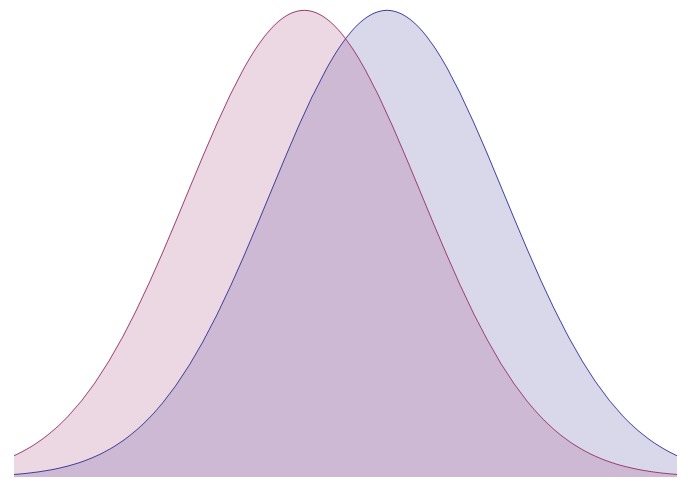
\includegraphics[width=0.8\linewidth]{{./figures/scan_symbol_no_axes}.eps}
  \end{center}
\end{figure}

\vfill

\hspace*{0.2in}\emph {University of California, Riverside} \ 
               \hspace{0.25in} {\bf Mike Beaumier}, {\bf Ken Barish}, {\bf Richard Hollis}

\hspace*{0.2in}\emph {STAR Experiment} \ 
               \hspace{0.25in} {\bf K. Oleg Eyser} \
\renewcommand*\familydefault{\rmdefault}



\clearpage

\pagestyle{fancy}

%==============================================  Excecutive Summary
\chapter{Introduction and Executive Summary}
\label{ch:intro}
The Vernier Scan Analysis is typically done every year, its purpose is to calculate the
absolute luminosity of collisions delivered to PHENIX's interaction region (IR) by RHIC.
Absolute luminosity is a necessary for the normalization of any cross-section (but not
necessary for cross-section ratos).  

The vernier analysis is done on a very special data set - obtained during a vernier scan.
Unlike normal data taking, PHENIX must use a special trigger configuration optimized for
recording very low rates of minimum bias data. The vernier scan itself consists of either
the blue, or yellow beams, being incrementally scanned across the other stationary beam.
If we assume that the blue and yellow beams are identical, this scan will effecitively
show us the transverse dimensions of the blue and yellow beams - these dimenions are used
to calculate the luminosity, $\mathcal{L}$, and to verify that our model for relativistic
beam collisions is correct.

We can also use the vernier scan to calibrate the Beam Beam Counters (BBC) in order to use
them as luminosity monitors. For any BBC trigger, we can represent the relationship
between $\mathcal{L}$ and the cross section observed by the BBC as:

\begin{equation} 
\label{eq:lumi_xsec_simple} 
\mathcal{L}_{BBC} = {R_{BBC}\over\sigma_{BBC}} 
\end{equation}

Where $\mathcal{L}_{BBC}$ is the effective luminosity delivered to a specific BBC trigger,
$R_{BBC}$ is the live event rate of the BBC trigger, and $\sigma_{BBC}$ is defined as the
cumulative cross section of events measured by this trigger.

The absolute luminosity is calculated as:

\begin{equation} 
\label{eq:lumi_one_bunch} 
\mathcal{L} = {f_{bunch}N_{b} N_{y}\over{2\pi\sigma_{x}\sigma_{y}}} 
\end{equation}

Where $\mathcal{L}$ is the luminosity, $f_{bunch}$ is the frequency of each individual
bunch crossing, $N_{b}, N_{y}$ are the bunch populations for the specific blue and yellow
beams, resepectively, and $\sigma_{x}, \sigma_{y}$ are the transverse widths both bunches
in the x and y directions. We assume identical beam bunch distributions for the blue and
yellow beams ~\cite{an888}, however individual bunches can also be studied - and this
analysis is presented in this note. $f_{bunch}$ corresponds to the bunch crossing rate of
a single specific bunch, and depends on the number of bunches in a specific fill and the
blue beam clock.

For clarity: The blue beam clock ticks once every time there is a bunch crossing.
Therefore, for $120$ bunch fills (including filled and empty bunches), and the standard
blue beam clock frequency, $f_{clock}$, of $9.36 MHz$, $f_{bunch} \equiv f_{clock} / 120 =
78 kHz$.

Previous analysis notes on the vernier analysis are listed below for benefit/curiosity of
the reader:

\begin{itemize}
\item AN184~\cite{an184}
\item AN597~\cite{an597}
\item AN688~\cite{an688}
\item AN888~\cite{an888}
\end{itemize}

Global vernier scan characteristics are summarized in table
~\ref{tab:global_scan_summary}. Each vernier scan is done slightly differently as a
systematic check - beam scan order is varied, beam energy is varied, scan length and step
length is varied, and sscanning patterns are varied. We expect that these variations will
not affect our final result.

\begin{sidewaystable}
\centering
\begin{tabular}{ccccccccc}
\toprule
\textbf{Run}    & \textbf{Fill}   & \textbf{Energy}          & \textbf{Scan}       & \textbf{Scan}    & \textbf{Scan}  & \textbf{Beam}    &                & \textbf{Step}     \\
\textbf{Number} & \textbf{Number} & \textbf{($GeV\sqrt{s}$)} & \textbf{Time (min)} & \textbf{Pattern} & \textbf{Order} & \textbf{Scanned} & \textbf{Steps} & \textbf{Time (s)} \\
\midrule
359711 & 16444 & 200 & 41 & Type 1 & H - V & Blue  & 26 & 57.5 \\
360879 & 16470 & 200 & 41 & Type 1 & H - V & Yellow& 26 & 61.2 \\
362492 & 16514 & 200 & 50 & Type 1 & V - H & Blue  & 26 & 62.3 \\
364636 & 16587 & 510 & 58 & Type 2 & H - V & Yellow& 18 & 21.7 \\
365866 & 16625 & 510 & 53 & Type 1 & H - V & Blue  & 26 & 70.0 \\
366605 & 16655 & 510 & 54 & Type 1 & H - V & Yellow& 26 & 67.7 \\
367138 & 16671 & 510 & 54 & Type 1 & H - V & Blue  & 26 & 68.65\\
\bottomrule
\end{tabular}
\caption{ A summary of vernier scans in run 12 }
\label{tab:global_scan_summary}
\end{sidewaystable}

\begin{figure}
\begin{center}
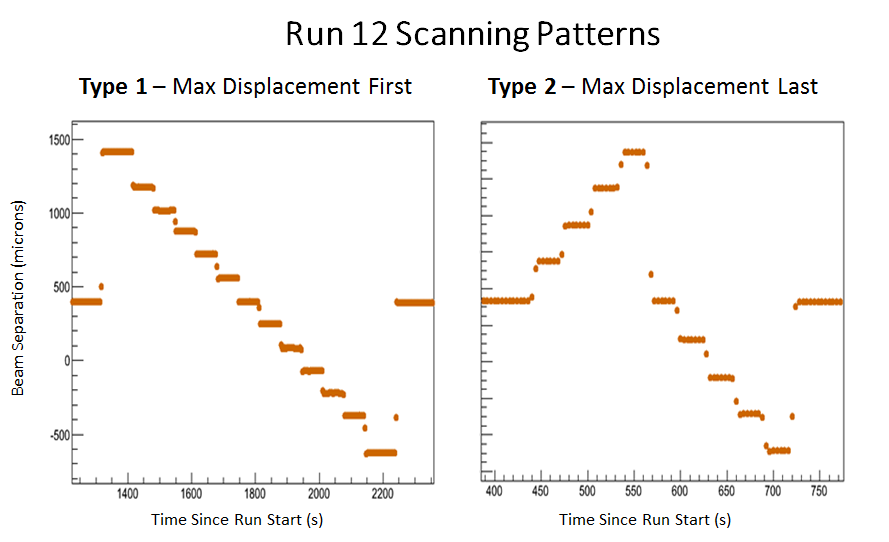
\includegraphics[width=0.75\linewidth]{./figures/scan_patterns}
\caption{ Two different scanning patterns were used in Run 12. Type 2 was previously
used in past years prior to 2012, and is included in this year's set of scans as a consistency check.
Type 1 was used for the majority of the scans in 2012. The scan order introduces
systematic effects based on rate losses in the beam width calculation, which are described
later.}
\label{fig:scan_patterns}
\end{center}
\end{figure}


\setcounter{page}{1}

\clearpage

\resetlinenumber

\clearpage

\resetlinenumber

\tableofcontents

\clearpage

\resetlinenumber
